\section{Kontextdiagramme}

\textbf{Kontextdiagramme} liefern eine grafische Übersicht der Systeme in ihrem Kontext.\\
Die Systeme selber werden dabei ohne innere Struktur dargestellt. da diese erst bei \textbf{Architektur} und \textbf{Entwurf} festgelegt wird.\\
Ein Kontextdiagramm zeigt darüber hinaus Schnittstellen zu anderen Systemen oder auch Anwendern und stellt die wichtigsten Anwendungsfälle dar.\\

\noindent
Als Notation für Kontextdiagramme werden i.d.R. \textbf{UML-Use-Case-Diagramme} benutzt, wobei Systeme als Pakete dargestellt werden, bei denen ihr Datenfluss durch Pfeile mit Richtungsangaben dargestellt wird (s. Abbildung~\ref{fig:usecaseexample}).

\begin{figure}
    \centering
    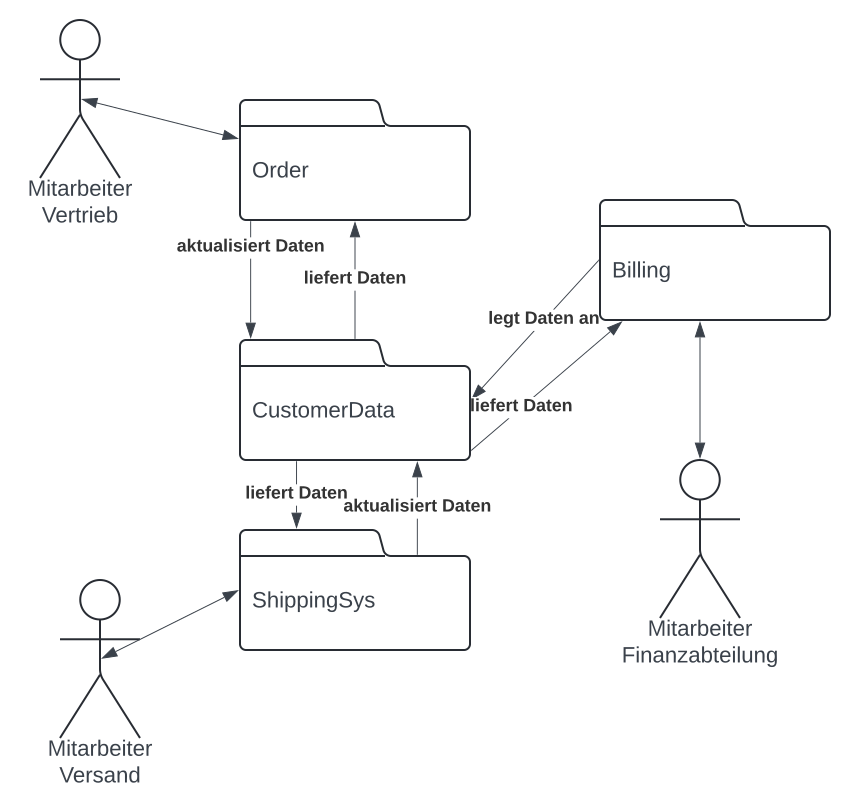
\includegraphics[scale=0.4]{chapters/Requirements Engineering/img/usecaseexample}
    \caption{Beispiel für ein Kontextdiagramm. (Quelle: eigene)}
    \label{fig:usecaseexample}
\end{figure}
